\documentclass{report}

\documentclass[12pt]{article}
\usepackage{array}
\usepackage{color}
\usepackage{amsthm}
\usepackage{eufrak}
\usepackage{lipsum}
\usepackage{pifont}
\usepackage{yfonts}
\usepackage{amsmath}
\usepackage{amssymb}
\usepackage{ccfonts}
\usepackage{comment} \usepackage{amsfonts}
\usepackage{fancyhdr}
\usepackage{graphicx}
\usepackage{listings}
\usepackage{mathrsfs}
\usepackage{setspace}
\usepackage{textcomp}
\usepackage{blindtext}
\usepackage{enumerate}
\usepackage{microtype}
\usepackage{xfakebold}
\usepackage{kantlipsum}
%\usepackage{draftwatermark}
\usepackage[spanish]{babel}
\usepackage[margin=1.5cm, top=2cm, bottom=2cm]{geometry}
\usepackage[framemethod=tikz]{mdframed}
\usepackage[colorlinks=true,citecolor=blue,linkcolor=red,urlcolor=magenta]{hyperref}

%//////////////////////////////////////////////////////
% Watermark configuration
%//////////////////////////////////////////////////////
%\SetWatermarkScale{4}
%\SetWatermarkColor{black}
%\SetWatermarkLightness{0.95}
%\SetWatermarkText{\texttt{Watermark}}

%//////////////////////////////////////////////////////
% Frame configuration
%//////////////////////////////////////////////////////
\newmdenv[tikzsetting={draw=gray,fill=white,fill opacity=0},backgroundcolor=none]{Frame}

%//////////////////////////////////////////////////////
% Font style configuration
%//////////////////////////////////////////////////////
\renewcommand{\familydefault}{\ttdefault}
\renewcommand{\rmdefault}{tt}

%//////////////////////////////////////////////////////
% Bold configuration
%//////////////////////////////////////////////////////
\newcommand{\fbseries}{\unskip\setBold\aftergroup\unsetBold\aftergroup\ignorespaces}
\makeatletter
\newcommand{\setBoldness}[1]{\def\fake@bold{#1}}
\makeatother

%//////////////////////////////////////////////////////
% Default font configuration
%//////////////////////////////////////////////////////
\DeclareFontFamily{\encodingdefault}{\ttdefault}{%
  \hyphenchar\font=\defaulthyphenchar
  \fontdimen2\font=0.33333em
  \fontdimen3\font=0.16667em
  \fontdimen4\font=0.11111em
  \fontdimen7\font=0.11111em}


%From M275 "Topology" at SJSU
\newcommand{\id}{\mathrm{id}}
\newcommand{\taking}[1]{\xrightarrow{#1}}
\newcommand{\inv}{^{-1}}

%From M170 "Introduction to Graph Theory" at SJSU
\DeclareMathOperator{\diam}{diam}
\DeclareMathOperator{\ord}{ord}
\newcommand{\defeq}{\overset{\mathrm{def}}{=}}

%From the USAMO .tex files
\newcommand{\ts}{\textsuperscript}
\newcommand{\dg}{^\circ}
\newcommand{\ii}{\item}

% % From Math 55 and Math 145 at Harvard
% \newenvironment{subproof}[1][Proof]{%
% \begin{proof}[#1] \renewcommand{\qedsymbol}{$\blacksquare$}}%
% {\end{proof}}

\newcommand{\liff}{\leftrightarrow}
\newcommand{\lthen}{\rightarrow}
\newcommand{\opname}{\operatorname}
\newcommand{\surjto}{\twoheadrightarrow}
\newcommand{\injto}{\hookrightarrow}
\newcommand{\On}{\mathrm{On}} % ordinals
\DeclareMathOperator{\img}{im} % Image
\DeclareMathOperator{\Img}{Im} % Image
\DeclareMathOperator{\coker}{coker} % Cokernel
\DeclareMathOperator{\Coker}{Coker} % Cokernel
\DeclareMathOperator{\Ker}{Ker} % Kernel
\DeclareMathOperator{\rank}{rank}
\DeclareMathOperator{\Spec}{Spec} % spectrum
\DeclareMathOperator{\Tr}{Tr} % trace
\DeclareMathOperator{\pr}{pr} % projection
\DeclareMathOperator{\ext}{ext} % extension
\DeclareMathOperator{\pred}{pred} % predecessor
\DeclareMathOperator{\dom}{dom} % domain
\DeclareMathOperator{\ran}{ran} % range
\DeclareMathOperator{\Hom}{Hom} % homomorphism
\DeclareMathOperator{\Mor}{Mor} % morphisms
\DeclareMathOperator{\End}{End} % endomorphism

\newcommand{\eps}{\epsilon}
\newcommand{\veps}{\varepsilon}
\newcommand{\ol}{\overline}
\newcommand{\ul}{\underline}
\newcommand{\wt}{\widetilde}
\newcommand{\wh}{\widehat}
\newcommand{\vocab}[1]{\textbf{\color{blue} #1}}
\providecommand{\half}{\frac{1}{2}}
\newcommand{\dang}{\measuredangle} %% Directed angle
\newcommand{\ray}[1]{\overrightarrow{#1}}
\newcommand{\seg}[1]{\overline{#1}}
\newcommand{\arc}[1]{\wideparen{#1}}
\DeclareMathOperator{\cis}{cis}
\DeclareMathOperator*{\lcm}{lcm}
\DeclareMathOperator*{\argmin}{arg min}
\DeclareMathOperator*{\argmax}{arg max}
\newcommand{\cycsum}{\sum_{\mathrm{cyc}}}
\newcommand{\symsum}{\sum_{\mathrm{sym}}}
\newcommand{\cycprod}{\prod_{\mathrm{cyc}}}
\newcommand{\symprod}{\prod_{\mathrm{sym}}}
\newcommand{\Qed}{\begin{flushright}\qed\end{flushright}}
\newcommand{\parinn}{\setlength{\parindent}{1cm}}
\newcommand{\parinf}{\setlength{\parindent}{0cm}}
% \newcommand{\norm}{\|\cdot\|}
\newcommand{\inorm}{\norm_{\infty}}
\newcommand{\opensets}{\{V_{\alpha}\}_{\alpha\in I}}
\newcommand{\oset}{V_{\alpha}}
\newcommand{\opset}[1]{V_{\alpha_{#1}}}
\newcommand{\lub}{\text{lub}}
\newcommand{\del}[2]{\frac{\partial #1}{\partial #2}}
\newcommand{\Del}[3]{\frac{\partial^{#1} #2}{\partial^{#1} #3}}
\newcommand{\deld}[2]{\dfrac{\partial #1}{\partial #2}}
\newcommand{\Deld}[3]{\dfrac{\partial^{#1} #2}{\partial^{#1} #3}}
\newcommand{\lm}{\lambda}
\newcommand{\uin}{\mathbin{\rotatebox[origin=c]{90}{$\in$}}}
\newcommand{\usubset}{\mathbin{\rotatebox[origin=c]{90}{$\subset$}}}
\newcommand{\lt}{\left}
\newcommand{\rt}{\right}
\newcommand{\paren}[1]{\left(#1\right)}
\newcommand{\bs}[1]{\boldsymbol{#1}}
\newcommand{\exs}{\exists}
\newcommand{\st}{\strut}
\newcommand{\dps}[1]{\displaystyle{#1}}

\newcommand{\sol}{\setlength{\parindent}{0cm}\textbf{\textit{Solution:}}\setlength{\parindent}{1cm} }
\newcommand{\solve}[1]{\setlength{\parindent}{0cm}\textbf{\textit{Solution: }}\setlength{\parindent}{1cm}#1 \Qed}

% Things Lie
\newcommand{\kb}{\mathfrak b}
\newcommand{\kg}{\mathfrak g}
\newcommand{\kh}{\mathfrak h}
\newcommand{\kn}{\mathfrak n}
\newcommand{\ku}{\mathfrak u}
\newcommand{\kz}{\mathfrak z}
\DeclareMathOperator{\Ext}{Ext} % Ext functor
\DeclareMathOperator{\Tor}{Tor} % Tor functor
\newcommand{\gl}{\opname{\mathfrak{gl}}} % frak gl group
\renewcommand{\sl}{\opname{\mathfrak{sl}}} % frak sl group chktex 6

% More script letters etc.
\newcommand{\SA}{\mathcal A}
\newcommand{\SB}{\mathcal B}
\newcommand{\SC}{\mathcal C}
\newcommand{\SF}{\mathcal F}
\newcommand{\SG}{\mathcal G}
\newcommand{\SH}{\mathcal H}
\newcommand{\OO}{\mathcal O}

\newcommand{\SCA}{\mathscr A}
\newcommand{\SCB}{\mathscr B}
\newcommand{\SCC}{\mathscr C}
\newcommand{\SCD}{\mathscr D}
\newcommand{\SCE}{\mathscr E}
\newcommand{\SCF}{\mathscr F}
\newcommand{\SCG}{\mathscr G}
\newcommand{\SCH}{\mathscr H}

% Mathfrak primes
\newcommand{\km}{\mathfrak m}
\newcommand{\kp}{\mathfrak p}
\newcommand{\kq}{\mathfrak q}

% number sets
\newcommand{\RR}[1][]{\ensuremath{\ifstrempty{#1}{\mathbb{R}}{\mathbb{R}^{#1}}}}
\newcommand{\NN}[1][]{\ensuremath{\ifstrempty{#1}{\mathbb{N}}{\mathbb{N}^{#1}}}}
\newcommand{\ZZ}[1][]{\ensuremath{\ifstrempty{#1}{\mathbb{Z}}{\mathbb{Z}^{#1}}}}
\newcommand{\QQ}[1][]{\ensuremath{\ifstrempty{#1}{\mathbb{Q}}{\mathbb{Q}^{#1}}}}
\newcommand{\CC}[1][]{\ensuremath{\ifstrempty{#1}{\mathbb{C}}{\mathbb{C}^{#1}}}}
\newcommand{\PP}[1][]{\ensuremath{\ifstrempty{#1}{\mathbb{P}}{\mathbb{P}^{#1}}}}
\newcommand{\HH}[1][]{\ensuremath{\ifstrempty{#1}{\mathbb{H}}{\mathbb{H}^{#1}}}}
\newcommand{\FF}[1][]{\ensuremath{\ifstrempty{#1}{\mathbb{F}}{\mathbb{F}^{#1}}}}
% expected value
\newcommand{\EE}{\ensuremath{\mathbb{E}}}
\newcommand{\charin}{\text{ char }}
\DeclareMathOperator{\sign}{sign}
\DeclareMathOperator{\Aut}{Aut}
\DeclareMathOperator{\Inn}{Inn}
\DeclareMathOperator{\Syl}{Syl}
\DeclareMathOperator{\Gal}{Gal}
\DeclareMathOperator{\GL}{GL} % General linear group
\DeclareMathOperator{\SL}{SL} % Special linear group

%---------------------------------------
% BlackBoard Math Fonts :-
%---------------------------------------

%Captital Letters
\newcommand{\bbA}{\mathbb{A}}	\newcommand{\bbB}{\mathbb{B}}
\newcommand{\bbC}{\mathbb{C}}	\newcommand{\bbD}{\mathbb{D}}
\newcommand{\bbE}{\mathbb{E}}	\newcommand{\bbF}{\mathbb{F}}
\newcommand{\bbG}{\mathbb{G}}	\newcommand{\bbH}{\mathbb{H}}
\newcommand{\bbI}{\mathbb{I}}	\newcommand{\bbJ}{\mathbb{J}}
\newcommand{\bbK}{\mathbb{K}}	\newcommand{\bbL}{\mathbb{L}}
\newcommand{\bbM}{\mathbb{M}}	\newcommand{\bbN}{\mathbb{N}}
\newcommand{\bbO}{\mathbb{O}}	\newcommand{\bbP}{\mathbb{P}}
\newcommand{\bbQ}{\mathbb{Q}}	\newcommand{\bbR}{\mathbb{R}}
\newcommand{\bbS}{\mathbb{S}}	\newcommand{\bbT}{\mathbb{T}}
\newcommand{\bbU}{\mathbb{U}}	\newcommand{\bbV}{\mathbb{V}}
\newcommand{\bbW}{\mathbb{W}}	\newcommand{\bbX}{\mathbb{X}}
\newcommand{\bbY}{\mathbb{Y}}	\newcommand{\bbZ}{\mathbb{Z}}

%---------------------------------------
% MathCal Fonts :-
%---------------------------------------

%Captital Letters
\newcommand{\mcA}{\mathcal{A}}	\newcommand{\mcB}{\mathcal{B}}
\newcommand{\mcC}{\mathcal{C}}	\newcommand{\mcD}{\mathcal{D}}
\newcommand{\mcE}{\mathcal{E}}	\newcommand{\mcF}{\mathcal{F}}
\newcommand{\mcG}{\mathcal{G}}	\newcommand{\mcH}{\mathcal{H}}
\newcommand{\mcI}{\mathcal{I}}	\newcommand{\mcJ}{\mathcal{J}}
\newcommand{\mcK}{\mathcal{K}}	\newcommand{\mcL}{\mathcal{L}}
\newcommand{\mcM}{\mathcal{M}}	\newcommand{\mcN}{\mathcal{N}}
\newcommand{\mcO}{\mathcal{O}}	\newcommand{\mcP}{\mathcal{P}}
\newcommand{\mcQ}{\mathcal{Q}}	\newcommand{\mcR}{\mathcal{R}}
\newcommand{\mcS}{\mathcal{S}}	\newcommand{\mcT}{\mathcal{T}}
\newcommand{\mcU}{\mathcal{U}}	\newcommand{\mcV}{\mathcal{V}}
\newcommand{\mcW}{\mathcal{W}}	\newcommand{\mcX}{\mathcal{X}}
\newcommand{\mcY}{\mathcal{Y}}	\newcommand{\mcZ}{\mathcal{Z}}


%---------------------------------------
% Bold Math Fonts :-
%---------------------------------------

%Captital Letters
\newcommand{\bmA}{\boldsymbol{A}}	\newcommand{\bmB}{\boldsymbol{B}}
\newcommand{\bmC}{\boldsymbol{C}}	\newcommand{\bmD}{\boldsymbol{D}}
\newcommand{\bmE}{\boldsymbol{E}}	\newcommand{\bmF}{\boldsymbol{F}}
\newcommand{\bmG}{\boldsymbol{G}}	\newcommand{\bmH}{\boldsymbol{H}}
\newcommand{\bmI}{\boldsymbol{I}}	\newcommand{\bmJ}{\boldsymbol{J}}
\newcommand{\bmK}{\boldsymbol{K}}	\newcommand{\bmL}{\boldsymbol{L}}
\newcommand{\bmM}{\boldsymbol{M}}	\newcommand{\bmN}{\boldsymbol{N}}
\newcommand{\bmO}{\boldsymbol{O}}	\newcommand{\bmP}{\boldsymbol{P}}
\newcommand{\bmQ}{\boldsymbol{Q}}	\newcommand{\bmR}{\boldsymbol{R}}
\newcommand{\bmS}{\boldsymbol{S}}	\newcommand{\bmT}{\boldsymbol{T}}
\newcommand{\bmU}{\boldsymbol{U}}	\newcommand{\bmV}{\boldsymbol{V}}
\newcommand{\bmW}{\boldsymbol{W}}	\newcommand{\bmX}{\boldsymbol{X}}
\newcommand{\bmY}{\boldsymbol{Y}}	\newcommand{\bmZ}{\boldsymbol{Z}}
%Small Letters
\newcommand{\bma}{\boldsymbol{a}}	\newcommand{\bmb}{\boldsymbol{b}}
\newcommand{\bmc}{\boldsymbol{c}}	\newcommand{\bmd}{\boldsymbol{d}}
\newcommand{\bme}{\boldsymbol{e}}	\newcommand{\bmf}{\boldsymbol{f}}
\newcommand{\bmg}{\boldsymbol{g}}	\newcommand{\bmh}{\boldsymbol{h}}
\newcommand{\bmi}{\boldsymbol{i}}	\newcommand{\bmj}{\boldsymbol{j}}
\newcommand{\bmk}{\boldsymbol{k}}	\newcommand{\bml}{\boldsymbol{l}}
\newcommand{\bmm}{\boldsymbol{m}}	\newcommand{\bmn}{\boldsymbol{n}}
\newcommand{\bmo}{\boldsymbol{o}}	\newcommand{\bmp}{\boldsymbol{p}}
\newcommand{\bmq}{\boldsymbol{q}}	\newcommand{\bmr}{\boldsymbol{r}}
\newcommand{\bms}{\boldsymbol{s}}	\newcommand{\bmt}{\boldsymbol{t}}
\newcommand{\bmu}{\boldsymbol{u}}	\newcommand{\bmv}{\boldsymbol{v}}
\newcommand{\bmw}{\boldsymbol{w}}	\newcommand{\bmx}{\boldsymbol{x}}
\newcommand{\bmy}{\boldsymbol{y}}	\newcommand{\bmz}{\boldsymbol{z}}

%---------------------------------------
% Scr Math Fonts :-
%---------------------------------------

\newcommand{\sA}{{\mathscr{A}}}   \newcommand{\sB}{{\mathscr{B}}}
\newcommand{\sC}{{\mathscr{C}}}   \newcommand{\sD}{{\mathscr{D}}}
\newcommand{\sE}{{\mathscr{E}}}   \newcommand{\sF}{{\mathscr{F}}}
\newcommand{\sG}{{\mathscr{G}}}   \newcommand{\sH}{{\mathscr{H}}}
\newcommand{\sI}{{\mathscr{I}}}   \newcommand{\sJ}{{\mathscr{J}}}
\newcommand{\sK}{{\mathscr{K}}}   \newcommand{\sL}{{\mathscr{L}}}
\newcommand{\sM}{{\mathscr{M}}}   \newcommand{\sN}{{\mathscr{N}}}
\newcommand{\sO}{{\mathscr{O}}}   \newcommand{\sP}{{\mathscr{P}}}
\newcommand{\sQ}{{\mathscr{Q}}}   \newcommand{\sR}{{\mathscr{R}}}
\newcommand{\sS}{{\mathscr{S}}}   \newcommand{\sT}{{\mathscr{T}}}
\newcommand{\sU}{{\mathscr{U}}}   \newcommand{\sV}{{\mathscr{V}}}
\newcommand{\sW}{{\mathscr{W}}}   \newcommand{\sX}{{\mathscr{X}}}
\newcommand{\sY}{{\mathscr{Y}}}   \newcommand{\sZ}{{\mathscr{Z}}}


%---------------------------------------
% Math Fraktur Font
%---------------------------------------

%Captital Letters
\newcommand{\mfA}{\mathfrak{A}}	\newcommand{\mfB}{\mathfrak{B}}
\newcommand{\mfC}{\mathfrak{C}}	\newcommand{\mfD}{\mathfrak{D}}
\newcommand{\mfE}{\mathfrak{E}}	\newcommand{\mfF}{\mathfrak{F}}
\newcommand{\mfG}{\mathfrak{G}}	\newcommand{\mfH}{\mathfrak{H}}
\newcommand{\mfI}{\mathfrak{I}}	\newcommand{\mfJ}{\mathfrak{J}}
\newcommand{\mfK}{\mathfrak{K}}	\newcommand{\mfL}{\mathfrak{L}}
\newcommand{\mfM}{\mathfrak{M}}	\newcommand{\mfN}{\mathfrak{N}}
\newcommand{\mfO}{\mathfrak{O}}	\newcommand{\mfP}{\mathfrak{P}}
\newcommand{\mfQ}{\mathfrak{Q}}	\newcommand{\mfR}{\mathfrak{R}}
\newcommand{\mfS}{\mathfrak{S}}	\newcommand{\mfT}{\mathfrak{T}}
\newcommand{\mfU}{\mathfrak{U}}	\newcommand{\mfV}{\mathfrak{V}}
\newcommand{\mfW}{\mathfrak{W}}	\newcommand{\mfX}{\mathfrak{X}}
\newcommand{\mfY}{\mathfrak{Y}}	\newcommand{\mfZ}{\mathfrak{Z}}
%Small Letters
\newcommand{\mfa}{\mathfrak{a}}	\newcommand{\mfb}{\mathfrak{b}}
\newcommand{\mfc}{\mathfrak{c}}	\newcommand{\mfd}{\mathfrak{d}}
\newcommand{\mfe}{\mathfrak{e}}	\newcommand{\mff}{\mathfrak{f}}
\newcommand{\mfg}{\mathfrak{g}}	\newcommand{\mfh}{\mathfrak{h}}
\newcommand{\mfi}{\mathfrak{i}}	\newcommand{\mfj}{\mathfrak{j}}
\newcommand{\mfk}{\mathfrak{k}}	\newcommand{\mfl}{\mathfrak{l}}
\newcommand{\mfm}{\mathfrak{m}}	\newcommand{\mfn}{\mathfrak{n}}
\newcommand{\mfo}{\mathfrak{o}}	\newcommand{\mfp}{\mathfrak{p}}
\newcommand{\mfq}{\mathfrak{q}}	\newcommand{\mfr}{\mathfrak{r}}
\newcommand{\mfs}{\mathfrak{s}}	\newcommand{\mft}{\mathfrak{t}}
\newcommand{\mfu}{\mathfrak{u}}	\newcommand{\mfv}{\mathfrak{v}}
\newcommand{\mfw}{\mathfrak{w}}	\newcommand{\mfx}{\mathfrak{x}}
\newcommand{\mfy}{\mathfrak{y}}	\newcommand{\mfz}{\mathfrak{z}}

\usepackage{minted}


\title{\Huge{Diseño y Análisis de Algoritmos}\\Tarea 4}
\author{\huge{Sergio Montoya Ramírez}}
\date{}

\begin{document}

\maketitle
\newpage% or \cleardoublepage
% \pdfbookmark[<level>]{<title>}{<dest>}
\pdfbookmark[section]{\contentsname}{toc}
\tableofcontents
\pagebreak

\chapter{Pregunta 1}

\section{Código}
\begin{minted}{java}
  /* Dynamic Programming Java implementation of Coin
  Change problem */
  import java.util.Arrays;

  class CoinChange {
    static long count(int coins[], int n, int sum)
    {
      // dp[i] will be storing the number of solutions for
      // value i. We need sum+1 rows as the dp is
      // constructed in bottom up manner using the base case
      // (sum = 0)
      int dp[] = new int[sum + 1];

      // Base case (If given value is 0)
      dp[0] = 1;

      // Pick all coins one by one and update the dp[]
      // values after the index greater than or equal to the
      // value of the picked coin
      for (int i = 0; i < n; i++)
      for (int j = coins[i]; j <= sum; j++)
      dp[j] += dp[j - coins[i]];

      return dp[sum];
      }

      // Driver Function to test above function
      public static void main(String args[])
      {
	int coins[] = { 1, 2, 3 };
	int n = coins.length;
	int sum = 5;
	System.out.println(count(coins, n, sum));
      }
      }
      // This code is contributed by Pankaj Kumar
\end{minted}

\section{Recurrencia}

En este caso, la recurrencia que utiliza por cada numero menor a $sum$, sumar la cantidad de maneras en las que se puede llegar a $sum$ desde este numero. Esto lo hace en cada paso sumando la cantidad de maneras que se puede llegar a la resta entre un $sum$ y el numero en el que se esta.

\section{Explicación}

\begin{enumerate}
  \item $coins:$ Este es el array en donde están las monedas. Básicamente nos dice que números podemos acceder.
  \item  $n$ : Este es el tamaño del Array en donde están las monedas. Básicamente, nos dice cuantos números distintos vamos a poder combinar.
  \item $sum$: Este es el objetivo al que debemos llegar. 
  \item $dp$: Este es un array que va a guardar todas las maneras en las que se pueda llegar a el numero $i$. En particular $dp[i]$ es este numero de veces.
  \item $i$ : Este es un contador que nos permite revisar el valor por cada moneda. Es decir, vamos a tener que iniciar el proceso recursivo en alguna parte y esta variable nos permite iniciar desde el valor de cada una de las monedas que están en el array $coins$.
  \item $j$: Esta es la variable que va a ir cambiando, básicamente cada ciclo lo que va a hacer es iniciar desde el valor que tenga $coins[i]$ y a partir de ahí recorrerá todos los valores menores a $sum$ sumando las posibilidades que tiene la diferencia entre $j$ y la moneda que se tiene.A
\end{enumerate}

\section{Diagrama Necesidades}

Es difícil dibujar el diagrama de necesidades pues depende seriamente de las monedas que tengamos. Basicamente para cada punto se debe sumar de todos los puntos anteriores de diferencia con la moneda que se tenga. El diagrama que aqui se va a exponer va a mostrarse como si solo ubiera dos monedas $1, 2$ pero es sumamente dependiente de la cantidad y el valor de cada moneda.

\begin{figure}[H]
  \centering
  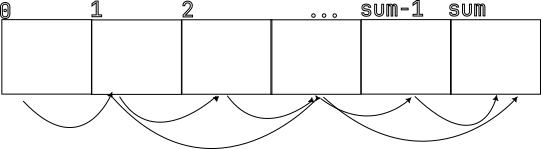
\includegraphics[width=0.8\textwidth]{img/necesidades_1.png}
  \caption{Diagrama de necesidades con dos monedas.}
  \label{fig:fig1}
\end{figure}

\section{Complejidad Temporal}

Revisemos linea a linea:
\begin{minted}{java}
  static long count(int coins[], int n, int sum) {
    int dp[] = new int[sum + 1]; // C1 | 1
    dp[0] = 1; // C2 | 1
    for (int i = 0; i < n; i++) // C3 | n
    for (int j = coins[i]; j <= sum; j++) // C4 | n*sum
    dp[j] += dp[j - coins[i]]; // C5 | n*sum
    return dp[sum]; // C6 | 1
    }
\end{minted}

Con lo cual el total queda:
\begin{align*}
  T\left( n, sum \right) &= C_1 + C_2 + C_3\cdot n + C_4 \cdot n\cdot sum + C_5\cdot n\cdot sum + C_6 \\
			 &= O\left( n\cdot sum \right)
		       .\end{align*}

		       \section{Complejidad Espacial}

		       En este caso, vamos a utilizar no solo las variables normales que son constantes si no ademas, se hará uso de un array con tamaño $sum + 1$. Por lo tanto, la complejidad espacial es:
		       \begin{align*}
			 E\left( n, sum \right) &= O\left( sum \right)  \\
		       .\end{align*}

		       \section{Ejemplos}

		       \begin{minted}{java}
  @Test
  public void primerTest() {
    int[] coins = {1, 2, 3, 4, 5};
    int n = coins.length;
    int sum = 20;
    long manerasSumar20 = CoinChange.count(coins, n, sum);
    assert manerasSumar20 == 192: String.format(
    "Algoritmo: %d | Respuesta: %d",
    manerasSumar20,
    192);
  }

  @Test
  public void segundoTest() {
    int[] coins = {1, 2, 5, 10, 20, 50, 100};
    int n = coins.length;
    int sum = 200;
    long manerasSumar200 = CoinChange.count(coins, n, sum);
    assert manerasSumar200 == 73681: String.format(
    "Algoritmo: %d | Respuesta: %d",
    manerasSumar200,
    73681);
  }
		       \end{minted}

		       \chapter{Pregunta 2}

		       \section{Código}
		       \begin{minted}{java}
  // Java Solution

  public class LongestPalinSubstring {

    // A utility function to print
    // a substring str[low..high]
    static void printSubStr(
    String str, int low, int high)
    {
      System.out.println(
      str.substring(
      low, high + 1));
    }

    // This function prints the longest
    // palindrome substring of str[].
    // It also returns the length of the
    // longest palindrome
    static int longestPalSubstr(String str)
    {
      // Get length of input string
      int n = str.length();

      // table[i][j] will be false if
      // substring str[i..j] is not palindrome.
      // Else table[i][j] will be true
      boolean table[][] = new boolean[n][n];

      // All substrings of length 1 are palindromes
      int maxLength = 1;
      for (int i = 0; i < n; ++i)
      table[i][i] = true;

      // Check for sub-string of length 2.
      int start = 0;
      for (int i = 0; i < n - 1; ++i) {
	if (str.charAt(i) == str.charAt(i + 1)) {
	  table[i][i + 1] = true;
	  start = i;
	  maxLength = 2;
	}
      }

      // Check for lengths greater than 2.
      // k is length of substring
      for (int k = 3; k <= n; ++k) {

	// Fix the starting index
	for (int i = 0; i < n - k + 1; ++i) {

	  // Get the ending index of substring from
	  // starting index i and length k
	  int j = i + k - 1;

	  // Checking for sub-string from ith index to
	  // jth index if str.charAt(i+1) to
	  // str.charAt(j-1) is a palindrome
	  if (table[i + 1][j - 1]
	  && str.charAt(i) == str.charAt(j)) {
	    table[i][j] = true;

	    if (k > maxLength) {
	      start = i;
	      maxLength = k;
	    }
	  }
	}
      }
      System.out.print("Longest palindrome substring is: ");
      printSubStr(str, start,
      start + maxLength - 1);

      // Return length of LPS
      return maxLength;
    }

    // Driver code
    public static void main(String[] args)
    {
      String str = "forgeeksskeegfor";
      System.out.println("Length is: " + longestPalSubstr(str));
    }
    }

    // This code is contributed by Sumit Ghosh
		       \end{minted}

		       \section{Recurrencia}

		       Básicamente lo que hace es primero revisa todos los palíndromos que hay de tamaño 2 y los pone en la matriz. Luego, revisa cada uno de esos y va expandiendo con respecto al tamaño. Es decir que va a probando con substratos cada vez mas grandes.

		       \section{Explicación}
		       \begin{enumerate}
			 \item $n$: tamaño completo del string.
			 \item $table$: matriz  $n\times n$ en la cual la posición $table[i][j]$ es verdadero si el substring $string[i..j]$ es palíndromo.
			 \item $maxLength$: Máximo tamaño del substring que se esta buscando. También pasa eventualmente a ser el valor mas grande de un substring que es palíndromo.
			 \item $start$ punto en el que inicia la búsqueda de palíndromos 
		       \end{enumerate}

		       Sin embargo, esto no deja muy claro el como funciona como tal. Por lo tanto miraremos con un poco mas de profundidad el siguiente loop.
		       \begin{minted}{java}
      for (int k = 3; k <= n; ++k) {
	for (int i = 0; i < n - k + 1; ++i) {
	  int j = i + k - 1;
	  if (table[i + 1][j - 1]
	  && str.charAt(i) == str.charAt(j)) {
	    table[i][j] = true;

	    if (k > maxLength) {
	      start = i;
	      maxLength = k;
	    }
	  }
	}
		       \end{minted}

		       Este loop básicamente va iterando desde 3 (que es el palíndromo mas pequeño que no se a revisado previamente) y mira si existe un palíndromo anterior que este yuxtapuesto a esta posición y repite este proceso hasta que reviso todos los posibles substrings.

		       \section{Diagrama Necesidades}

		       \section{Complejidad Temporal}

		       Revisemos linea a linea:
		       \begin{minted}{java}
    static int longestPalSubstr(String str)
    {
      int n = str.length(); // C1 | 1
      boolean table[][] = new boolean[n][n]; // C2 | 1
      int maxLength = 1; // C3 | 1
      for (int i = 0; i < n; ++i) // C4 | n
	table[i][i] = true; // C5 | n
      int start = 0; // C6 | 1
      for (int i = 0; i < n - 1; ++i) { // C7 | n - 1
	if (str.charAt(i) == str.charAt(i + 1)) {  // C8 | n - 1
	  table[i][i + 1] = true; // C9 | n - 1
	  start = i; // C10 | n - 1
	  maxLength = 2; // C11 | n - 1
	}
      }
      for (int k = 3; k <= n; ++k) { // C12 | n - 2
	for (int i = 0; i < n - k + 1; ++i) { // C13 | n^2
	  int j = i + k - 1; // C14 | n^2
	  if (table[i + 1][j - 1] // C15 | n^2
	  && str.charAt(i) == str.charAt(j)) { // C16 | n^2
	    table[i][j] = true; // C17 | n^2
	    if (k > maxLength) { // C18 | n^2
	      start = i; // C19 | n^2
	      maxLength = k; // C20 | n^2
	    }
	  }
	}
      }
      System.out.print("Longest palindrome substring is: "); // C21 | 1
      printSubStr(str, start, // C22 | 1
      start + maxLength - 1); // C23 | 1
      return maxLength; // C24 | 1
    }
		       \end{minted}

		       Por lo tanto la complejidad temporal seria:
		       \begin{align*}
			 T\left( n \right) &= C_1 + C_2 + C_3 + C_4\cdot n + C_5\cdot n + C_6 + \\
					   &\left( C_7 + C_8 + C_9 + C_{10} + C_{11} \right)  \left( n - 1 \right) + C_{12} \cdot n + \\
					   &\left( C_{13} + C_{14} + C_{15} + C_{16} + C_{17} + C_{18} + C_{19} + C_{20} \right)\cdot n^2 + C_{21} + C_{22} + C_{23} + C_{24} \\
			 T\left( n \right)  &= O\left( n^2 \right)  \\
		       .\end{align*}

		       \section{Complejidad Espacial}

		       En este caso todo es constante exceptuando la matriz $table$ que de hecho tiene tamaño  $n^2$ por lo tanto la complejidad espacial es: \[
			 E\left( n \right) = O\left( n^2 \right) 
		       .\] 

		       \section{Ejemplos}
		       \begin{minted}{java}
  @Test
  public void primerTest() {
    String str = "Esto es una prueba"
    int pal = LongestPalinSubstring.longestPalSubstr(str)
    assert pal == 1: String.format(
    "Algoritmo: %d | Respuesta: %d",
    pal,
    1);
  }

  @Test
  public void segundoTest() {
    String str = "Para probarraborp tenemos hannah"
    int pal = LongestPalinSubstring.longestPalSubstr(str)
    assert pal == 14: String.format(
    "Algoritmo: %d | Respuesta: %d",
    pal,
    14);
  }
  \end{minted}
\end{document}
